\documentclass[leqno]{article}
\usepackage[margin=0.5in]{geometry}
\usepackage[utf8]{inputenc}
\usepackage{amsmath, amsfonts, color, booktabs, centernot, graphicx, fancyhdr}
\usepackage[linktoc=all,hidelinks]{hyperref}
\setlength\parindent{0pt}
\begin{document}
\title{Markov Chain Model of Genetic Evolution: EE 126 Project 1}
\author{Ajeya Cotra, Leah Dickstein, Davis Foote, Ena Hariyoshi}

\maketitle
 
\setlength{\parskip}{\baselineskip}

Our project uses a Markov chain to model the genetic evolution of the peppered moth ({\it Biston betularia}) over the last two hundred years.

\section{Background}

The dramatic changes the species underwent in a relatively short evolutionary time span make the peppered moth one of the most well-studied and celebrated creatures in evolutionary biology. {\it Biston betularia}, native to England, started off mostly white, to camouflage with the light trees and lichen in its environment:

\begin{center}
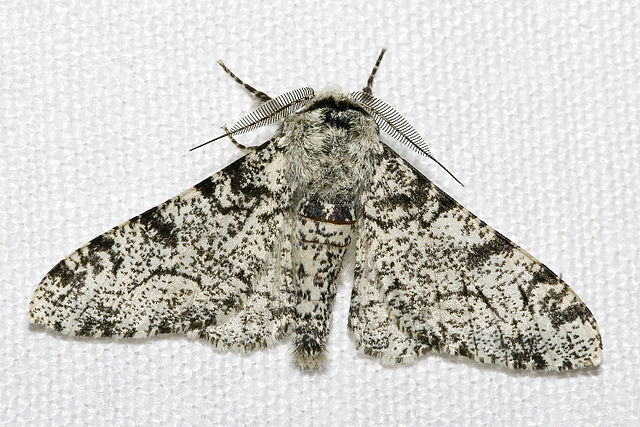
\includegraphics[scale=0.8]{white_peppered_moth.jpg}{\\White peppered moth, {\it Biston betularia f. typica}.}
\end{center}

However, with the advent of the industrial revolution, increased pollution in the moths' habitats killed off most lichen and stained light-colored trees with soot, causing white moths to stand out against the darkened environment. The previously advantageous coloring now made lighter moths more visible to predators. Over the next several decades, white peppered moths were almost completely eliminated from the population and {\it Biston betularia} became dark gray colored:

\begin{center}
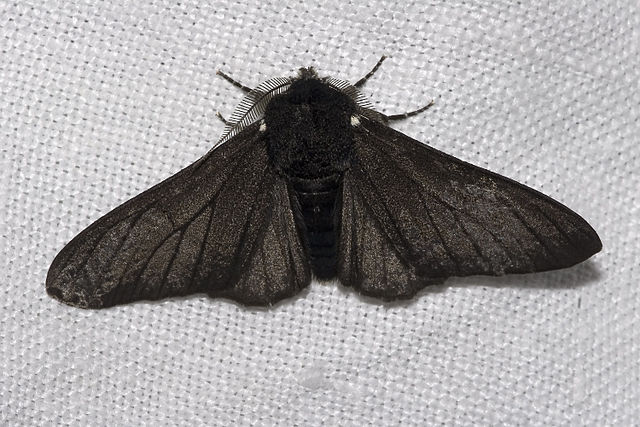
\includegraphics{black_peppered_moth.jpg}{\\Black peppered moth, {\it Biston betularia f. carbonaris}.}
\end{center}

The white peppered moth was virtually eliminated from the population in a very short time. This led us to wonder what evolutionary pressure would be necessary to have a high probability of fully eliminating a trait from a population within a fixed amount of time.

\newpage

\section{Simulation}

In our simulation, individual moths are either white or gray. Coloration is modeled as a Mendelian trait -- two alleles, $W$ and $g$, represent the white and gray traits respectively. Each moth has two color alleles which together determine its color. In our model, white is dominant, so $WW$ and $Wg$ mean the moth is white, while $gg$ means the moth is gray.

We model a moth population as a discrete time Markov chain whose states represent the number of $WW$, $Wg$, and $gg$ moths in the population (for example, in an experiment with population $45$, the state may record $15$ $WW$ moths, $23$ $Wg$ moths, and $7$ $gg$ moths at time $k$). At each time step, the population experiences exactly one birth and one death, detailed in the transition model below.

\subsection{Transition Model}

Let $N$ be the total number of moths in the population. Because at each time step we have exactly one birth and one death, $N$ remains stable. Define $N_{ww}$ to be the number of $WW$ moths, $N_{wg}$ to be the number of $Wg$ moths, and $N_{gg}$ to be the number of $gg$ moths. At time $k$, our state $X_k$ is represented as $\{N_{ww},\ N_{wg},\ N_{gg}\}$. 

\textbf{Birth}

To transition, we begin with the birth phase. Two moths are chosen at random from the current population. One allele is randomly selected from each parent to produce an offspring moth. The probability of each offspring genotype given parent genotypes are given in the table below:

\begin{tabular}{c|c|c|c|c|c|c|} \cline{2-7} 
{} & \multicolumn{6}{|c|}
{Parent genotypes}\\
\hline
\multicolumn{1}{|c|}{Offspring genotype} & WW, WW & WW, Wg & WW, gg & Wg, Wg & Wg, gg & gg, gg\\
\hline
\multicolumn{1}{|c|}{WW} & 1 & 1/2 & 0 & 1/4 & 0 & 0\\
\multicolumn{1}{|c|}{Wg} & 0 & 1/2 & 1 & 1/2 & 1/2 & 0\\
\multicolumn{1}{|c|}{gg} & 0 & 0 & 0 & 1/4 & 1/2 & 1\\
\hline
\multicolumn{1}{|c|}{Total} & $\left(\frac{N_{ww}}{N}\right)^2$ & $2\left(\frac{N_{ww}}{N}\right)\left(\frac{N_{wg}}{N}\right)$ & $2\left(\frac{N_{ww}}{N}\right)\left(\frac{N_{gg}}{N}\right)$ & $\left(\frac{N_{wg}}{N}\right)^2$ & $2\left(\frac{N_{ww}}{N}\right)\left(\frac{N_{gg}}{N}\right)$ & $\left(\frac{N_{gg}}{N}\right)^2$ \\
\hline
\end{tabular}\\

Let $b_x$ be the probability that the offspring moth created has genotype $x$. From the table above we can calculate 

\begin{align*}
% b_{ww} &= \left\left(\frac{WW}{N} \right\right)^2 + \frac{WW\, gg}{N^2} + \frac{1}{4}\left\left(\frac{wg}{N}\right\right)^2\\
b_{ww}\ &=\ \frac{1}{N^2}\left((WW)^2\ +\ (WW)\, (gg)\ +\ \frac{1}{4}\, Wg\right)\\
% b_{wg} &= \frac{WW\, Wg}{N^2} + \frac{1}{2}\left\left(\frac{Wg\, gg}{N^2}\right\right) + \frac{1}{2}\left\left(\frac{Wg}{N}\right\right)^2 + 2\, \frac{WW\, gg}{N^2}\\
b_{wg}\ &=\ \frac{1}{N^2}\left( (WW)\, (Wg)\ +\ \frac{1}{2}\, (Wg)\, (gg)\ +\ \frac{1}{2}\, (Wg)^2\ +\ 2\, (WW)\, (gg) \right)\\
b_{gg}\ &=\ \frac{1}{N^2}\left((gg)^2\ +\ (gg)\, (Wg)\ +\ \frac{1}{4}\, (Wg)^2\right)
\end{align*}

Once a moth is born, we update $N$ and the appropriate count ($WW$, $Wg$, or $gg$) to reflect this.\\

\textbf{Death}

Following the birth of the offspring moth, we randomly select a moth from the entire population (including the new offspring) to kill before we transition to the next time step. The state at $k + 1$ will be the resulting count of $WW$, $Wg$, and $gg$ after {\it both} one birth and one death have occurred.

\newpage

Probability of death is determined by {\it phenotype} rather than genotype: a white moth has probability $d_{white}$ of death. Let $d_x$ be the probability that a moth of genotype $x$ is chosen to be killed. We can calculate the $d_x$ in terms of $d_{white}$ from the information above:

\begin{align*}
d_{ww}\ &=\ d_{white}\, P(WW \mid \text{white})\ &=\ d_{white}\, \left(\frac{WW}{WW\ +\ Wg}\right)\\
d_{wg}\ &=\ d_{white}\, P(Wg \mid \text{white})\ &=\ d_{white}\left(\frac{Wg}{WW\ +\ Wg}\right)\\
d_{gg}\ &=\ 1 - d_{white}
\end{align*}

\textbf{State Transitions}

If the Markov chain is in state $X_k\ =\ \{N_{ww},\ N_{wg},\ N_{gg}\}$ where $N_{ww},\, N_{wg},\ N_{gg}\ >\ 0$, then based on the birth and death in that state, there are $7$ possibilities for state $X_{k + 1}$: 

\begin{align*}
\{N_{ww} - 1,\ N_{wg} + 1,\ N_{gg}\} &\ \implies \text{ $Wg$ born, $WW$ died}\\
\{N_{ww} - 1,\ N_{wg},\ N_{gg} + 1\} &\ \implies \text{ $gg$ born, $WW$ died}\\
\{N_{ww} + 1,\ N_{wg} - 1,\ N_{gg}\} &\ \implies \text{ $WW$ born, $Wg$ died}\\
\{N_{ww},\ N_{wg} - 1,\ N_{gg} + 1\} &\ \implies \text{ $gg$ born, $Wg$ died}\\
\{N_{ww} + 1,\ N_{wg},\ N_{gg} - 1\} &\ \implies \text{ $WW$ born, $gg$ died}\\
\{N_{ww},\ N_{wg} + 1,\ N_{gg} - 1\} &\ \implies \text{ $Wg$ born, $gg$ died}\\
\{N_{ww},\ N_{wg},\ N_{gg}\} &\ \implies \text{ Same type born as died}
\end{align*}

If one or more of the $N_x$ is $0$, there are fewer transition possibilities. In particular, there are two absorbing states:

\begin{align*}
\{N_{ww} > 0,\ 0,\ 0\} &\ \implies \text{ Gray allele eliminated}\\
\{0,\ 0,\ N_{gg} > 0\} &\ \implies \text{ White allele eliminated}
\end{align*} 

The transition diagram below depicts the web of transitions visually for a population of size $3$:

\begin{center}
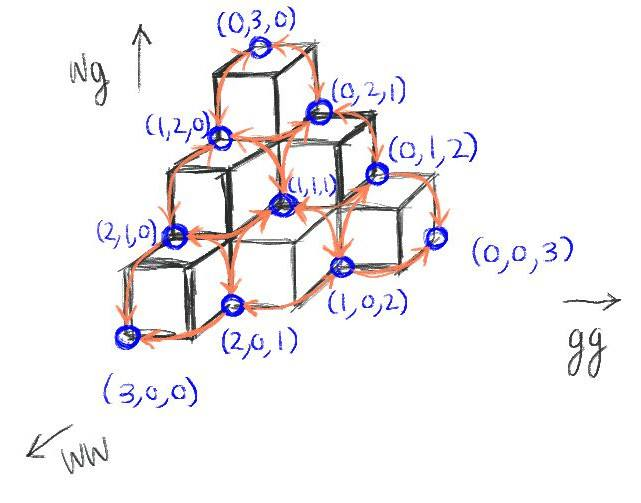
\includegraphics[width=3in]{transition_diagram.jpg}{\\States depicted in blue and transitions in orange.}
\end{center}

If transitioning into a particular state requires a moth of genotype $x$ to be born and a moth of genotype $y$ to be killed, the transition probability is simply $b_{x}\, d_{y}$.

\subsection{Python Implementation}

The project code can be found in the {\tt sim.py} file. The main function is {\tt simulate}, which takes in an {\tt initial\_state} and (optionally) {\tt prob\_white} and {\tt max\_steps}, which represent the probability that the moth killed in a given transition is white, and the number of time steps the program is allowed to simulate, respectively. If not provided, {\tt prob\_white} defaults to {\tt 0.9} and {\tt max\_steps} defaults to {\tt 10000}.

The {\tt simulate} function runs until it either reaches an absorbing state or has run {\tt max\_steps} times. If the population is entirely gray, it returns {\tt True}. If the population is entirely white or {\tt max\_steps} is reached before an absorbing state is reaching, it returns {\tt False}.

\textbf{State Representation}

States are represented as Python dictionaries of length $3$. The keys are genotypes, represented by the strings {\tt `ww'}, {\tt `wg'}, and {\tt `gg'}, and the values are the number of moths of that genotype. The user must input {\tt initial\_state} in that format. Population size is inferred by summing over the values of the dictionary, and is kept constant through the simulation.

\textbf{Birth and Death}

The code for birth is given in the {\tt new\_child} function, and the code for death is given in the {\tt kill\_moth} function.

It's important to note that the {\tt new\_child} partition moths into disjoint sets for mating; the simulation as written (and the analytic calculations we ran) assume any moth can mate with any moth. This does mean there is some probability that a moth may mate with itself. However, for larger population sizes this probability becomes negligible and does not affect the results very much.

The {\tt kill\_moth} function will kill white moths with probability {\tt prob\_white} and gray moths with probability {\tt 1\ -\ prob\_white} if both white and gray moths are present; if there are no gray moths, it will kill a white moth uniformly at random.

\newpage

\section{Results}

Lorem ipsum dolor sit amet, consectetur adipiscing elit. Mauris ultrices volutpat lorem sed elementum. Suspendisse mollis a orci tempus ultricies. Ut diam tortor, dignissim non lorem bibendum, dapibus congue nisl. Etiam elementum non nulla quis accumsan. 

Nam eget enim eget leo tristique dignissim. Aenean facilisis nibh ut ipsum vestibulum laoreet.Sed mollis congue metus, a molestie magna efficitur quis. Nam id odio eu mauris tincidunt vulputate sit amet eget sapien. Mauris mollis leo vel ante tristique mattis. 

Quisque interdum a nisl non viverra. Integer ac purus augue. Ut non convallis felis. Morbi eu urna diam. Curabitur tempus est non est consectetur, id viverra enim lacinia. Integer sed maximus lorem.

Lorem ipsum dolor sit amet, consectetur adipiscing elit. Mauris ultrices volutpat lorem sed elementum. Suspendisse mollis a orci tempus ultricies. Ut diam tortor, dignissim non lorem bibendum, dapibus congue nisl. 

Etiam elementum non nulla quis accumsan. Nam eget enim eget leo tristique dignissim. Aenean facilisis nibh ut ipsum vestibulum laoreet. Sed mollis congue metus, a molestie magna efficitur quis. Nam id odio eu mauris tincidunt vulputate sit amet eget sapien. 

Mauris mollis leo vel ante tristique mattis. Quisque interdum a nisl non viverra. Integer ac purus augue. Ut non convallis felis. Morbi eu urna diam. Curabitur tempus est non est consectetur, id viverra enim lacinia. Integer sed maximus lorem.

\end{document}